\let\negmedspace\undefined
\let\negthickspace\undefined
\documentclass[journal]{IEEEtran}
\usepackage[a5paper, margin=10mm, onecolumn]{geometry}
%\usepackage{lmodern} % Ensure lmodern is loaded for pdflatex
\usepackage{tfrupee} % Include tfrupee package

\setlength{\headheight}{1cm} % Set the height of the header box
\setlength{\headsep}{0mm}     % Set the distance between the header box and the top of the text
\usepackage{gvv-book}
\usepackage{gvv}
\usepackage{cite}
\usepackage{amsmath,amssymb,amsfonts,amsthm}
\usepackage{algorithmic}
\usepackage{graphicx}
\usepackage{textcomp}
\usepackage{xcolor}
\usepackage{txfonts}
\usepackage{listings}
\usepackage{enumitem}
\usepackage{mathtools}
\usepackage{gensymb}
\usepackage{comment}
\usepackage[breaklinks=true]{hyperref}
\usepackage{tkz-euclide} 
\usepackage{listings}
% \usepackage{gvv}                                        
\def\inputGnumericTable{}                                 
\usepackage[latin1]{inputenc}                                
\usepackage{color}                                            
\usepackage{array}                                            
\usepackage{longtable}                                       
\usepackage{calc}                                             
\usepackage{multirow}                                         
\usepackage{hhline}                                           
\usepackage{ifthen}                                           
\usepackage{lscape}



\usepackage{amsmath,amssymb}
\usepackage{booktabs}
\usepackage{tikz}
\usetikzlibrary{arrows.meta,angles,quotes}





\begin{document}

\bibliographystyle{IEEEtran}
\vspace{3cm}

\title{1.2.29}
\author{AI25BTECH11021 - Abhiram Reddy N}
% \maketitle
% \newpage
% \bigskip
{\let\newpage\relax\maketitle}

\renewcommand{\thefigure}{\theenumi}
\renewcommand{\thetable}{\theenumi}
\setlength{\intextsep}{10pt} % Space between text and floats


\numberwithin{equation}{enumi}
\numberwithin{figure}{enumi}
\renewcommand{\thetable}{\theenumi}


\textbf{Question}:\\The angles between
two vectors a and b with magnitude
$\sqrt{3}$ and 4, respectively,
and a, b= 2 $\sqrt{3}$ is


\section*{Angle Between Two Vectors}

Given:
\[
|\vec{a}| = \sqrt{3}, \quad |\vec{b}| = 4, \quad \vec{a} \cdot \vec{b} = 2\sqrt{3}
\]

\textbf{Formula for angle between two vectors:}
\[
\vec{a} \cdot \vec{b} = |\vec{a}| |\vec{b}| \cos\theta
\]

\textbf{Substitute values:}
\[
2\sqrt{3} = \sqrt{3} \cdot 4 \cdot \cos\theta = 4\sqrt{3} \cos\theta
\]

\[
\cos\theta = \frac{2\sqrt{3}}{4\sqrt{3}} = \frac{1}{2}
\]

\[
\theta = \cos^{-1}\left(\frac{1}{2}\right) = \boxed{60^\circ}
\]


\begin{figure}[htbp]
\centering
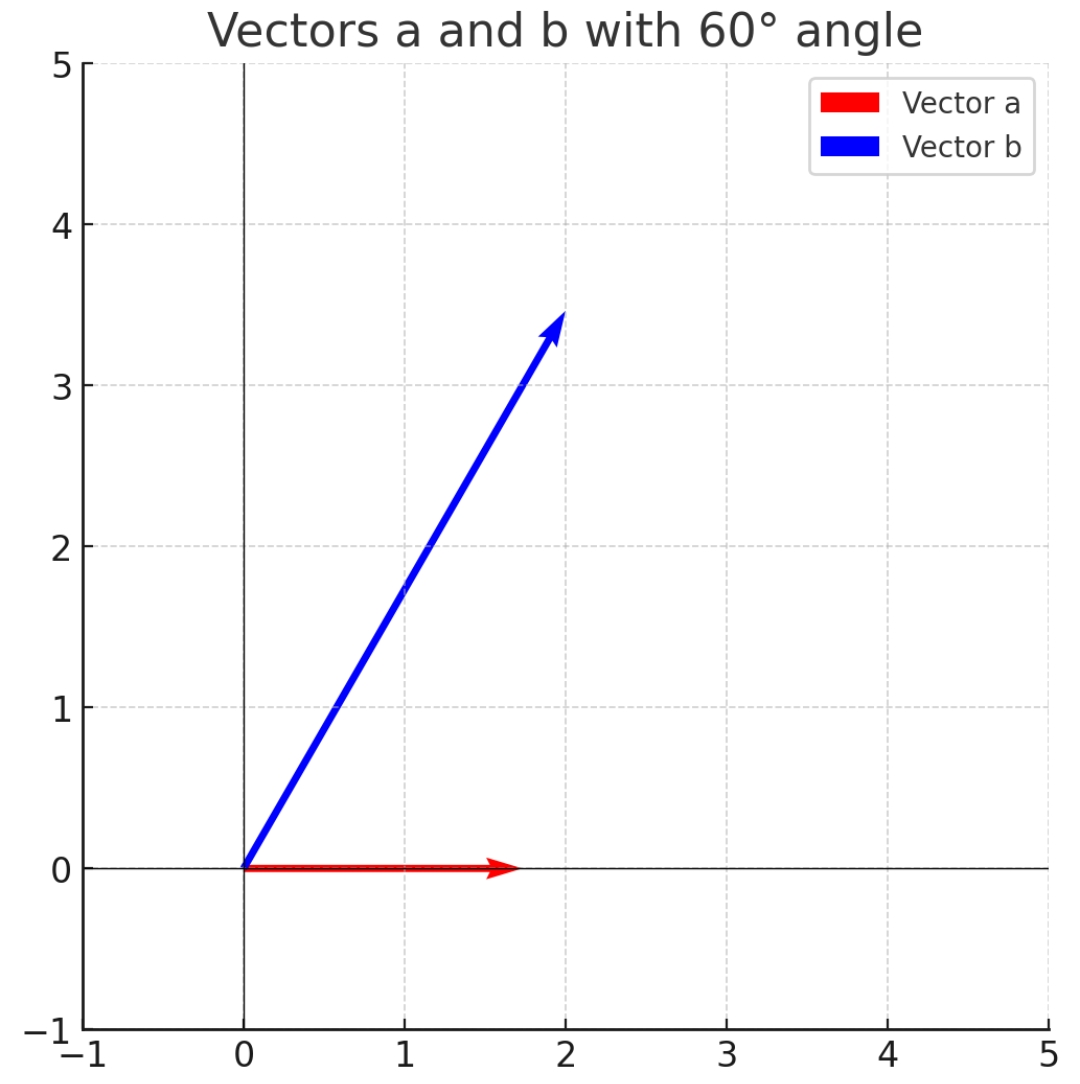
\includegraphics[width=0.8\columnwidth]{figs/python_plot.png} 
\caption{plot $\mathbf{R}$ obtained as $\mathbf{W}-\mathbf{V}$}
\label{fig:plot}
\end{figure}
















\end{document}
